
\section{Euler图与Hamilton图}
\subsection{Euler图与中国邮路问题}
\subsubsection{Euler图及其性质}
\begin{definition}
对于连通图$G$,如果$G$中存在经过每条边的闭
迹,则称$G$为\textcolor{red}{欧拉图},简称$G$为$E$图. \textcolor{red}{欧拉闭迹}又称为
欧拉环游,或欧拉回路. 对于连通图$G$,如果$G$中存在经过每条边的迹,则称该迹为G的一条\textcolor{red}{欧拉迹}.
\end{definition}
\begin{theorem}
	下列陈述对于非平凡连通图G是等价的:
	\begin{enumerate}
		\item $G$是欧拉图;
		\item $G$的顶点度数为偶数;
		\item $G$的边集合能划分为圈.
	\end{enumerate}
\end{theorem}
\begin{note}
	欧拉图一定没有割边,有可能有割点(联系例\ref{yyhng}).
\end{note}
\begin{corollary}
	\begin{enumerate}
		\item \colorbox{yellow}{连通图$G$是欧拉图当且仅当$G$的顶点度数为偶数.}
		\item \colorbox{yellow}{连通非欧拉图$G$存在欧拉迹当且仅当$G$中只有两
			个顶点度数为奇数.}
	\end{enumerate}
\end{corollary}
\begin{note}
	\begin{enumerate}
		\item 	欧拉图必存在欧拉迹,非欧拉图可能存在欧拉迹. 非平凡欧拉图一定有圈.
		\item   图 $G$ 有欧拉迹当且仅当 $G$ 能“一笔画”.若奇度点数为零,则一笔画与起点无关;若奇度点数为 2,则一笔画的起点与终点均为
		奇点.
	\end{enumerate}

	
	
	
\end{note}

\subsubsection{Fleury算法}
该算法解决了在欧拉图中求出一条具体欧拉环游的方
法.方法是尽可能\textcolor{red}{避割边行走}.
\noindent 算法步骤:
\begin{enumerate}
	\item 任意选择一个顶点$v_0$,置$w_0=v_0$;
	\item 假设迹$wi=v_0e_1v_1\cdots e_iv_i$已经选定,那么按下述方
	\label{hhhh}
	法从$E-\{e_1,e_2,\cdots,e_i\}$中选取边$e_{i+1}$:
	\begin{itemize}
		\item  \textcolor{red}{$e_{i+1}$与$v_i$相关联};
		\item 除非没有别的边可选择,否则$e_{i+1}$不能是
		$G_i=G-\{e_1,e_2,\cdots,e_i\}$的割边.
	\end{itemize}
	\item 当\ref{hhhh}不能进行时,停止.
\end{enumerate}

\begin{example}
	证明:若$G$有$2k>0$个奇数顶点,则存在$k$条边不重
	的迹$Q_1, Q_2, \cdots,Q_k$,使得:
	\[
	E(G) = E(Q_1)\cup E(Q_2) \cup \cdots \cup E(Q_k)
	\]
\end{example}
\begin{proof}
	不失一般性,只就$G$是连通图进行证明.
	
	设$G=(n,m)$是连通图. 令$v_1, v_2,\cdots, v_k, v_{k+1},\cdots, v_{2k}$是$G$的所有奇度点.
	
	在$v_i$与$v_{i+k}$间连新边$e_i$得图$G^{*}(1\leq i \leq k)$.则$G^{*}$是欧拉图,因此,由Fleury算法得欧拉环游C.
	
	在C中删去$e_i$ $(1\leq i \leq k)$.得k条边不重的迹$Q_i$ $(1\leq i \leq k)$:
		\[
	E(G) = E(Q_1)\cup E(Q_2) \cup \cdots \cup E(Q_k)
	\]
\end{proof}

\subsubsection{中国邮路问题}

针对边赋权图的非欧拉图.

\begin{theorem}
若$W$是包含图$G$的每条边至少一次的闭途径,则$W$具有最小权值当且仅当下列两个条件被满足:
	\begin{enumerate}
		\item \colorbox{yellow}{$G$的每条边在$W$中最多重复一次;}
		\item \colorbox{yellow}{对于$G$的每个圈上的边来说,在$W$中重复的边的总权
			值不超过该圈非重复边总权值.}
	\end{enumerate}
\end{theorem}
\begin{note}
	设图 $G$ 是具有 $k$ 个奇度顶点,则在 $G$ 中最少添加 $k/2$ 条边才能使 $G$ 具有欧
	拉回路.
\end{note}

\begin{example}
\textcolor{red}{如果一个非负权的边赋权图$G$中只有两个奇度顶点$u$与$v$,设计一个求其最优欧拉环游的算法.}

\noindent 解:
\noindent 算法步骤:
\begin{enumerate}
	\item 在$u$与$v$间求出一条最短路$P$; (最短路算法)
	\item 在最短路$P$上,给每条边添加一条平行边得$G$的欧
	拉母图$G^{*}$;
	\item 在$G$的欧拉母图$G^{*}$ 中用Fleury算法求出一条欧拉
	环游.
\end{enumerate}
\end{example}


\subsection{Hamilton图}
\begin{definition}
	对于连通图$G$,经过$G$中每个点仅一次的\textcolor{red}{圈(路)}称为$G$的\textcolor{red}{Hamilton圈(路)},
	存在Hamilton圈的图称为\colorbox{yellow}{\textcolor{red}{Hamilton图}},简称$H$图. Hamilton路简称$H$路.
\end{definition}
\begin{note}
	\textcolor{red}{$H$图可能有割点,如$K_3$加一个自环.}
\end{note}

\begin{theorem}[必要条件]
	\label{jjjjjhhhh}
	若$G$为$H$图,则对$V(G)$的任一非空顶点子集$S$,有:
	\[
	\colorbox{yellow}{$\omega(G-S)\leq |S|$}
	\]
\end{theorem}
\begin{proof}
	设$C$是$G$的$H$圈,则对$V(G)$的任意非空子集$S$,容易知道:
	\[
	\omega(C-S)\leq |S|
	\]
	又因$C-S$是$G-S$的生成子图,故有
	\[
	\omega(G-S)\leq \omega(C-S)\leq |S|.
	\]
\end{proof}
\begin{note}
	\textcolor{red}{不等式为$G$是$H$图的必要条件,即不等式不满足
		时,可断定对应图是非$H$图};但满足不等式,不一定是Hamilton图,如彼德森图.彼得森图不是$H$图,是超$H$图.
\end{note}

\begin{theorem}[充分条件]
	设$G$是$n(n\geq 3)$阶简单图,
	\begin{enumerate}
		\item \colorbox{yellow}{若$\delta\geq \frac{n}{2}$,则$G$是$H$图}(Dirac定理).
		\item  \colorbox{yellow}{若对$G$中任意不相邻顶点$u$和$v$,都有$d(u)+d(v)\geq n$,则$G$是$H$图}(Ore定理).
	\end{enumerate}
\end{theorem}

\begin{theorem}[充要条件](帮迪——闭包定理)
	图$G$是$H$图当且仅当它的闭包是$H$图.
\end{theorem}
\begin{corollary}[充分条件]
	\textcolor{red}{设$G$是$n(n\geq 3)$阶简单图,若图$G$的闭包$\hat{G}$是完全图,则$G$是$H$图}.
\end{corollary}
\begin{note}
	任意图 G 的闭包是唯一的.一个图的闭包不一定是完全图.
\end{note}


\begin{theorem}[充分条件]
	\label{jjjjch}
	设简单图$G$的度序列是$(d_1,d_2,\cdots,d_n)$, 这里,$d_1\leq d_2\leq \cdots \leq d_n$,并且$n\geq3$.若对任意
	的$m<\frac{n}{2}$,或有 $d_m>m$,或有$d_{n-m} \geq n-m$,则$G$是$H$图(且$G$的闭包为完全图).
\end{theorem}
\begin{example}
	教材P84例题对定理\ref{jjjjch}的应用
\end{example}



\subsection{度极大非Hamilton图}

\begin{definition}
图$G$称为\colorbox{yellow}{\textcolor{red}{度极大非$H$图}},如果它的度不弱
于其它非$H$图.
\end{definition}


\begin{definition}[$C_{m,n}$图]
	对于$1\leq m < \frac{n}{2}$,则
	\[
		\colorbox{yellow}{$C_{m,n} = K_m\lor(\overline{K}_m+K_{n-2m})$}
	\]
\end{definition}


\begin{lemma}
	对于$1\leq m < \frac{n}{2}$的图
\colorbox{yellow}{$C_{m,n} = K_m\lor(\overline{K}_m+K_{n-2m})$}是非$H$图.
\end{lemma}
\begin{proof}
	由定义知,在$C_{m,n}$中属于$K_m$的任意一点$v$,其度数均为$d(v)=m+(m-1)+(n-2m)=n-1$.若$S$是$K_m$的顶点集,则$\omega(C_{m,n}-S)=	m+1>|S|=m$,由定理\ref{jjjjjhhhh}知$C_{m,n}$是非$H$图.
\end{proof}

\begin{theorem}[Chvátal,1972]
	\label{jjjjsll}
\colorbox{yellow}{若$G$是$n\geq 3$的非$H$简单图,则$G$度弱于某个$C_{m,n}$图}.
\end{theorem}

\begin{proof}
	设$G$是度序列为$(d_1,d_2,\cdots, d_n)$的非$H$图,这里$d_1\leq d_2\leq \cdots\leq d_n, n\geq 3$. 由定理\ref{jjjjch}知,存在$m\geq \frac{n}{2}$使得$d_m\leq m$且$d_{n-m}<n-m$. 因此$G$的度序列弱于下列序列:
	\[
	(m,\cdots,n-m-1,\cdots,n-m-1, n-1,\cdots,n-1)
	\]
	这个序列有$m$项等于$m$,有$n-2m$项等于$n-m-1$,有$m$项等于$n-1$,因此它就是$C_{m,n}$的度序列.
\end{proof}
\begin{note}
\textcolor{red}{对于固定正整数$n$,只要$1\leq m < \frac{n}{2}$,则$C_{m,n}$均是度极大非$H$图,随$m$的不同取值就得到$n$点度极大非$H$图族.} 定理\ref{jjjjsll}的逆不成立,如: $5$ 阶圈 $C_5$ 的度序列是 $(2, 2, 2, 2, 2)$,它度弱于 $C_{2,5}$ 的度序列 $(2, 2, 2, 4, 4)$,但
$C_5$ 是 $H$ 图.
\end{note}
\begin{example}
	具有 $5$ 个点的度极大非哈密尔顿图族为 $C_{1,5}$ 和$ C_{2,5}$.
\end{example}


\begin{corollary}
设$G$是$n$阶单图. 若$n\geq 3$且$|E(G)|>C_{n-1}^2+1$则$G$是$H$图;并且,具有$n$个顶点和$C_{n-1}^2+1$条边的非$H$简单图只有$C_{1,n}$以及当$n=5$时还有$C_{2,5}$.
\end{corollary}
\begin{note}
	$n$ 阶完全图中 $H$ 圈的个数为 $(n - 1)!$.
\end{note}





\subsection{最优H圈}

在边赋权图中求最小$H$圈是NP一难问题.

\subsubsection{边交换技术(上界)}
在赋权完全图中取一个初始$H$圈$C$;将$H$圈$C$进行修改.

\subsubsection{最优$H$圈的下界}
\noindent 过程(考过):
\begin{enumerate}
	\item 在$G$中删掉一点$v$(任意的)得图$G_1$
	\item  在图$G_1$中求出一棵最小生成树$T$;
	\item 在$v$的关联边中选出两条权值最小者$e_1$与$e_2$.若$C$是$G$的最优$H$圈,则:
	\[
	 w(C)\geq w(T)+w(e_1)+w(e_2)
	\]
\end{enumerate}
\noindent 说明(考过):

设$C$是$G$的最优$H$圈,则对$G$中任意一点$v$,$C-v$是$G-v$的$H$路,也是$G-v$的生成树.由此推知: 设$T$是$G-v$最小生成树,同时选取与$v$关联的两条边$e_1, e_2$使得$w(e_1)+w(e_2)$尽可能小,则$w(T)+w(e_1)+w(e_2)$是$w(C)$的一个下界.

\subsection{E图和H图的联系}

\begin{figure}[H]
	\small
	\centering 
	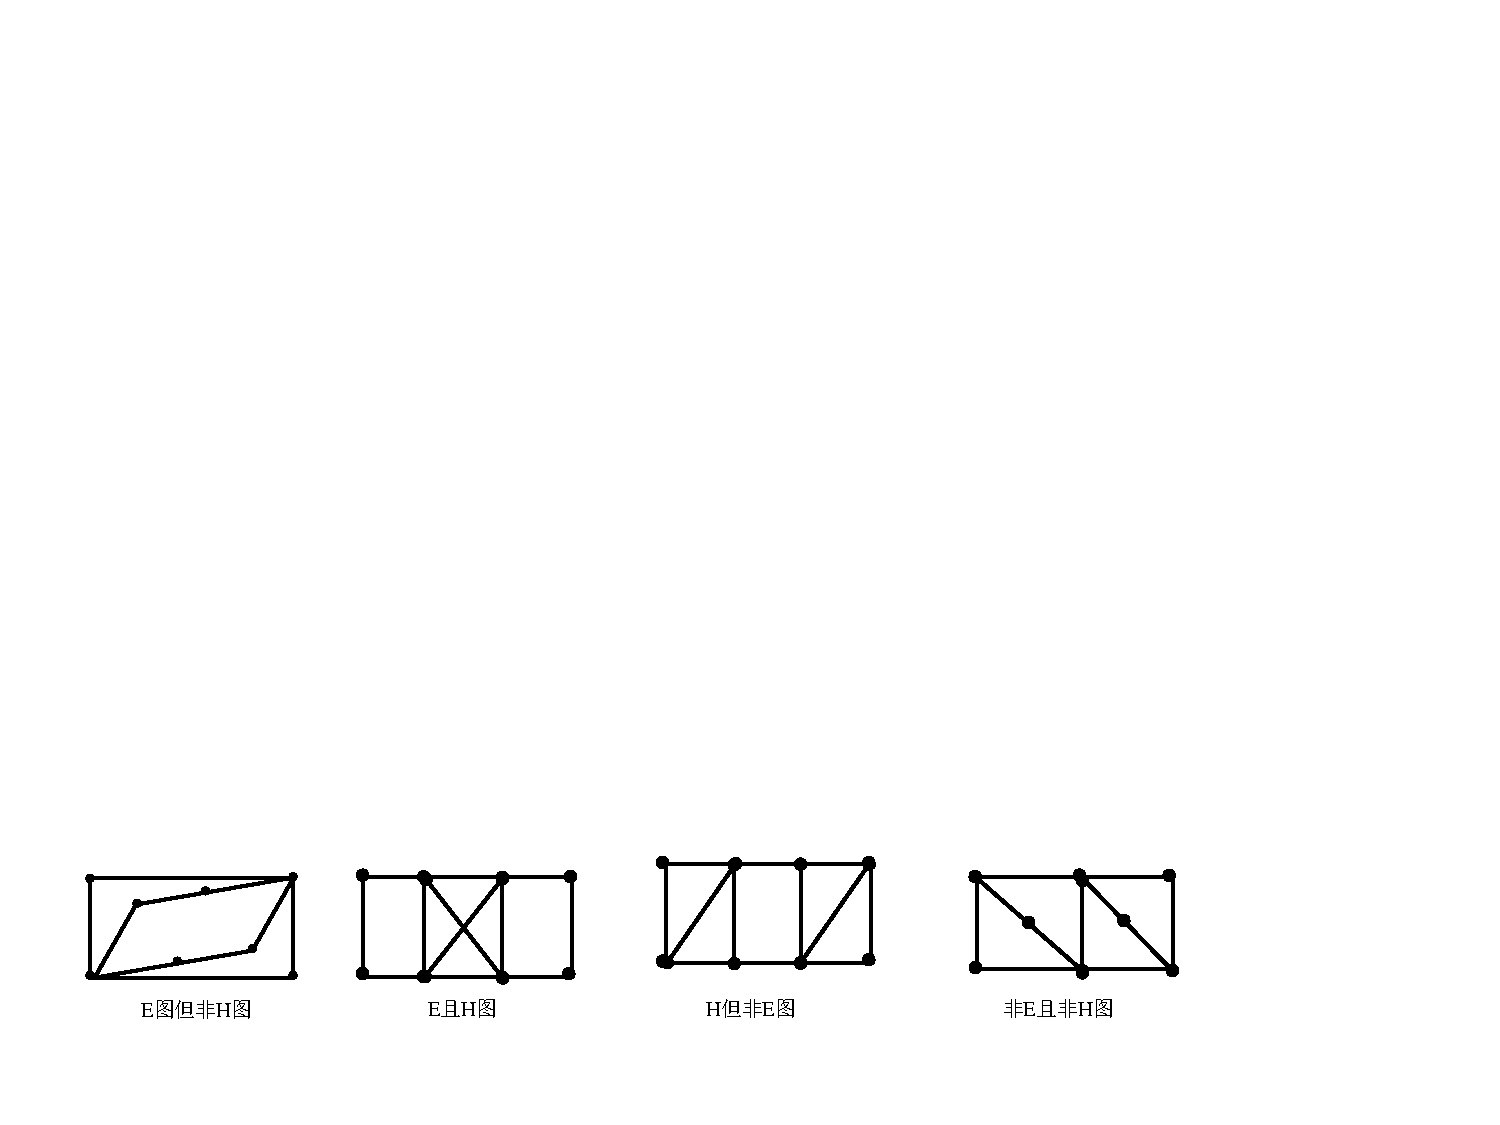
\includegraphics[scale=0.8]{image/CH4EH.pdf}  
	%\caption{信息包结构} 
	\label{figkjjj1ik}  
\end{figure}

\begin{definition}[线图]
设$G$是图,$G$的线图$L(G)$定义为:
	\begin{enumerate}
	\item \colorbox{yellow}{$V(L(G))=E(G)$};
	\item  \colorbox{yellow}{当$G$中两个边邻接时,$L(G)$的两个点邻接.}
\end{enumerate}
\end{definition}
一般地,\colorbox{yellow}{$L^{1}(G)=L(G), L^{2}(G)=L(L(G)),L^{n}(G)=L(L^{n-1}(G))$}

\begin{figure}[H]
	\small
	\centering 
	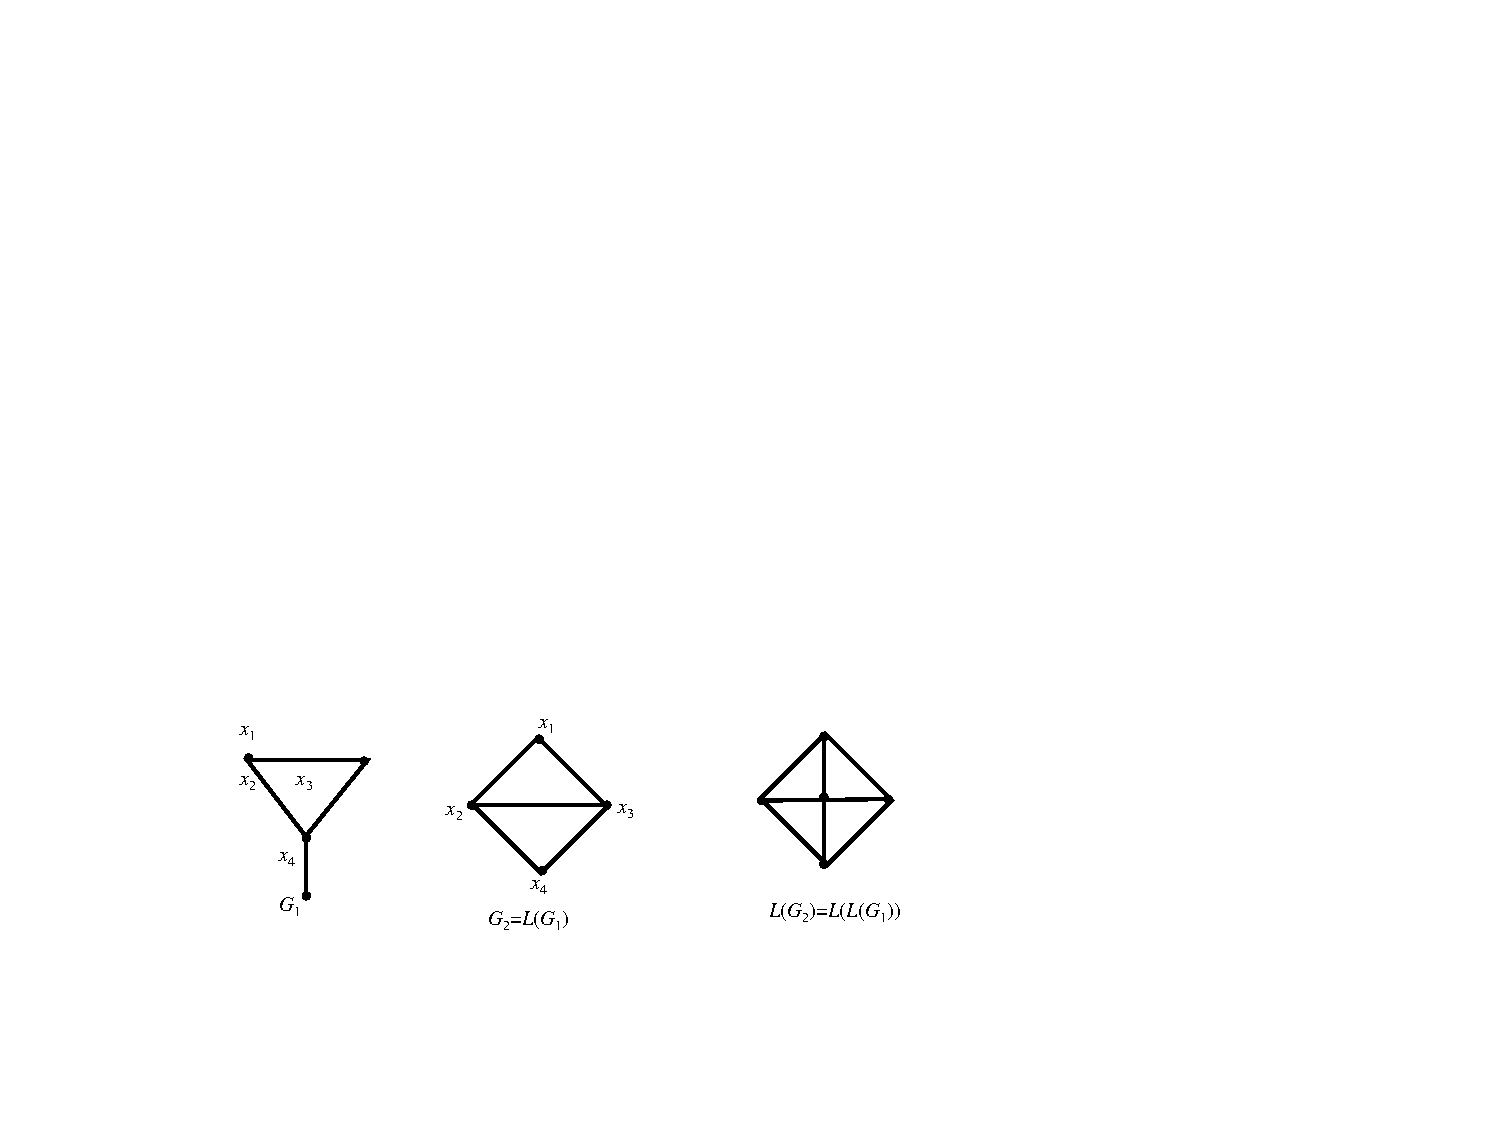
\includegraphics[scale=0.8]{image/CH4_LG.pdf}  
	%\caption{信息包结构} 
	\label{figkjjj1KKik}  
\end{figure}

\noindent {\bfseries \textcolor{ecolor}{线图的性质:}}

\begin{enumerate}
	\item 若$e=uv$是$G$的边,则$e$作为$L(G)$的顶点度数为;\colorbox{yellow}{$d(e) = d_G(u)+d_G(v)-2$};
	\item 若$G=(n, m)$, 则线图$L(G)$ 边数为:\colorbox{yellow}{$m(L(G))=-m+\frac{1}{2}\sum\limits_{v\in V(G)}d^2(v)$}.
\end{enumerate}


\begin{definition}
	称$S_n$是图$G$的$n$次细分图,是指将$G$的每条边中都
	插入$n$个$2$度顶点.\colorbox{yellow}{$L_n(G)=L(S_{n-1}(G))$}.
\end{definition}
\begin{note}
	\textcolor{red}{$L^{n}(G)\ne L_n(G)$}
\end{note}

\begin{theorem}
	\begin{enumerate}
	\item \colorbox{yellow}{若$G$是$E$图,则$L(G)$ 既是$E$图又是$H$图}.
	\item  \colorbox{yellow}{若$G$是$H$图,则$L(G)$是$H$图}
\end{enumerate}
\end{theorem}
\begin{note}
	该定理逆不成立.
\end{note}
\begin{theorem}
一个图$G$ 是$E$图的充要条件是$L_3(G)$为$H$图
\end{theorem}
\begin{theorem}[Chartarand]
若$G$ 是$n$个点的非平凡连通
图,且不是一条路,则对所有$m\geq n-3$,$L^m(G)$ 是$H$图
\end{theorem}








